
\documentclass[10pt]{extarticle}

\usepackage[headinclude=false,footinclude=false,%
	paper=A5,paper=landscape, pagesize]{typearea}
\usepackage{blindtext}
\usepackage[ngerman]{babel}
\usepackage[utf8]{inputenc}
\usepackage[T1]{fontenc}
\usepackage{graphicx} 
\usepackage{floatflt}
\usepackage{multicol}
\usepackage{enumitem} 
\usepackage[landscape]{geometry}

%Umgebung um ein Bild ordentlich in eine multicol-Umgebung zu setzen (das ist sonst nicht möglich)
\newenvironment{Figure}
  {\par\medskip\noindent\minipage{\linewidth}}
  {\endminipage\par\medskip}
\setlength{\parindent}{0in} 

\renewcommand{\familydefault}{\sfdefault}
%\areaset{19.4cm}{13.2cm}
\geometry{a5paper, top=5mm, left=8mm, right=8mm, bottom=10mm,
headsep=0mm, footskip=0mm}
\pagestyle{empty}
\begin{document}
\columnsep30pt
\begin{multicols}{2}

\subsection*{Weitere Fragen?}
Wenn es bei der Konfiguration irgendwelche Probleme gibt, könnt Ihr Euch jederzeit (am besten per Mail) bei uns melden. Natürlich könnt Ihr auch Euer gesamtes Zeug einpacken und bei uns vorbeikommen. Wir sind mittwochs ab 20 Uhr für Euch da. \\

\begin{tabular}{ll}
\textbf{Mail:} 			& freifunk@bingo-ev.de\\
\textbf{Telefon:}  	& 0841 9812368\\
\textbf{IRC:} 			& \#ffin auf hackint.net
\end{tabular}

\subsubsection*{Hier sind wir!}
Krumenauer Str. 54, 85049 Ingolstadt\\
In den Räumen des bytewerks auf der Rückseite des Gebäudes\\
direkt am Hollis-Parkplatz\\


\begin{Figure}
\centering
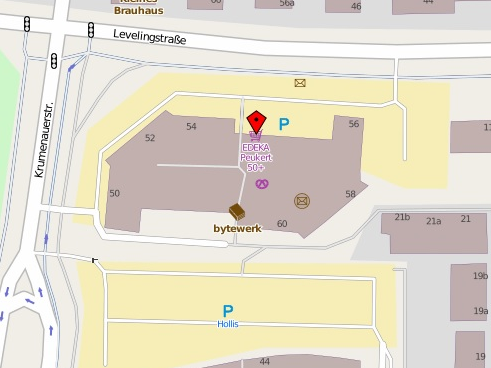
\includegraphics[width=0.8 \textwidth]{hiersindwir.png}
\end{Figure}

\columnbreak
\subsection*{Einrichtung Eures Routers}

Wenn Ihr einen fertig geflashten Router in den Händen haltet (direkt von uns), könnt Ihr diese Kurzanleitung benutzen. Ansonsten müsst Ihr den Router zuvor noch flashen. Eine ausführliche Anleitung dazu gibt es unter www.freifunk-ingolstadt.de/anleitung
\vfil
\subsection*{Vorbereitung}
Folgende Dinge sollten in Reichweite sein, wenn Ihr starten wollt:\\
\begin{itemize}
	\item Der fertig geflashte Router von uns, mit Netzteil für die Steckdose (liegt bei)
  \item Ein Netzwerkkabel (liegt dem Router bei)
  \item Einen eingeschalteten PC/Laptop mit Ethernetbuchse und einem Betriebssystem Eurer Wahl (Windows, MAC, Linux, …)
	\item Eine Internetverbindung via Ethernet oder einen anderer Freifunkrouter in der Nähe
\end{itemize}
\vfill
Eine Hilfe zur Konfiguration findet Ihr innen. 
\vfill
Euer Team von Freifunk Ingolstadt
\end {multicols}
\newpage

\subsection*{Freifunk-Firmware einmalig einrichten}
\columnsep20pt
\begin{multicols}{2}

\textbf{1. Schritt:} Ist der Router geflasht, müsst Ihr ihn lediglich mit Eurem PC verbinden. Dazu steckt Ihr das eine Ende des Netzwerkkabels in eine der LAN-Buchsen am Router (bei TP-Link gelb) und das andere in Euren PC. Jetzt könnt Ihr in einem Browser Eurer Wahl unter http://192.168.1.1/den Router konfigurieren. Es öffnet sich automatisch der Einrichtungs-Wizard, mit dem Ihr Daten, die Ihr teilen wollt, eingeben könnt. Eine Übersicht, über die Bedeutung der verschiedenen Felder:\\


\textbf{Name:} Den Namen könnt Ihr frei wählen, er taucht später auf der Knotenkarte auf. Ihr könnt diese Einstellung aber auch dekaktivieren.  \\

\textbf{Kontakt:} Hier könnt Ihr freiwillig eine Mailadresse angeben, damit wir oder andere Freifunker euch kontaktieren können. Freifunk lebt durch den Kontakt miteinander, denn so können wir zusammen ein stabiles Netz aufbauen. Bitte beachtet, dass die Mailadresse innerhalb des Freifunknetzes öffentlich ist.\\

\textbf{Mesh-VPN aktivieren:} Wenn Ihr Euer Internet für Freifunk zur Verfügung stellt, baut der Router mit Hilfe des Mesh-VPNs eine sichere VPN-Verbindung zu unserem Freifunk-Gateway auf. So können Knoten in der Nähe, ohne Mesh-VPN oder mit ausgefallener Internetverbindung, über Euren Router ins Internet gelangen.\\
Falls Eure Internetleitung nicht viel hergibt, könnt Ihr in diesem Unterpunkt auch einstellen, welche Kapazität von Eurem Internet Ihr anderen zur Verfügung stellt.\\

\columnbreak
\textbf{Knoten auf der Karte anzeigen:} Ein grafisches Schmankerl. Durch das Aktivieren dieser Einstellung kann man die Position Eures Freifunkrouters auf der Karte sehen. So kann die Verteilung von Freifunk besser verfolgt werden und Ihr könnt euch mit anderen Freifunkern absprechen, damit Eure Router meshen können. Das Meshnetz hält Freifunk stabil, auch wenn einmal ein Internetanschluss ausfallen sollte. Diese Funktion kann nach Belieben deaktiviert werden.\\
Der unter ‘Name’ gewählte Knotenname wird auf der Karte dort angezeigt, wo Ihr Eure Geokoordinaten setzt. Wenn Ihr das nicht wollt, könnt Ihr den nächsten Abschnitt überspringen.\\
Diese lassen sich über eine Kartensoftware, wie beispielsweise Google Maps, leicht abfragen, wenn Ihr an der passenden Stelle auf „Was ist hier” klickt.  \\

\textbf{Expertenoptionen:} \textit{Wichtig:} In den Expertenoptionen solltet Ihr nur etwas ändern, wenn Ihr Euch mit der Materie auskennt! Hier ist automatisch alles für den richtigen Betrieb eingestellt.\\

\textbf{2. Schritt:} Nun könnt Ihr Euren konfigurierten Router an ein Netzwerkkabel über die WAN-Buchse (bei TP-Link blau) mit dem Internet verbinden oder lasst Euren Router mit einem anderen Gerät in der Nähe automatisch verbinden (meshen). \\

\textbf{3. Schritt:} Jetzt könnt Ihr die Verbindung testen. Bitte etwas Geduld mitbringen: Bis zur ersten Verbindung kann es 10 Minuten dauern. \\


\vfill

Wenn alles klappt, seid Ihr fertig!
\end{multicols}
\end{document}
